\chapter{ส่วนประกอบต่าง ๆ ของภาษา Python}

\section{ตัวแปร (Variables)}

ตัวแปร (Variables) คือชื่อที่ผู้เขียนโปรแกรมกำหนดขึ้นมาเอง เพื่อใช้สำหรับการเก็บค่าข้อมูลในการเขียนโปรแกรมไว้ในหน่วยความจำของเครื่องคอมพิวเตอร์ โดยในภาษา Python ไม่ต้องระบุประเภทของตัวแปรไว้ในตอนที่ประกาศการตั้งชื่อตัวแปร

\begin{codelist}{การตั้งชื่อตัวแปร}{}
>>> a = 1
>>> a
1
>>> b = 2
>>> b
2
>>> a + b
3
>>> vat = 7
>>> vat
7
\end{codelist}

\section{การตั้งชื่อตัวแปร}

การตั้งชื่อตัวแปรสำหรับภาษา Python มีเงื่อนไขดังนี้

\begin{enumerate}[noitemsep]
\item ให้ขึ้นต้นด้วยอักษรตัวภาษาอังกฤษตัวใหญ่หรือตัวเล็กตั้งแต่ Aa ถึง Zz เท่านั้น 
\item ประกอบด้วยตัวอักษรหรือตัวเลข 0 ถึงเลข 9 หรือตัวขีดล่าง Underscore (\pyinline{_}) แต่ห้ามมีช่องว่าง
\item ตัวเลข 0-9 จะนำหน้าชื่อตัวแปรไม่ได้
\item ตัวพิมพ์เล็กและตัวพิมพ์ใหญ่เป็นตัวแปรคนละตัวกัน (Case-Sensitive) เช่น Name ไม่ใช่ตัวแปรเดียวกันกับ name 
\item ใช้ใส่เครื่องหมาย = ในการตั้งตัวแปรหรือให้ค่าแก่ตัวแปร
\item การตั้งชื่อตัวแปรควรตั้งอย่างสมเหตุสมผล 
\item ภาษา Python จะมีคำที่ถูกสงวนไว้ในการเขียนโปรแกรม หรือ Keywords ซึ่งห้ามนำมาใช้ในการตั้งชื่อตัวแปร ชื่อฟังก์ชัน หรือ ชื่อคลาส 
\end{enumerate}

\section{การตั้งชื่อตัวแปรพร้อมกันหลายตัวแปร}

ในการเขียนโปรแกรมภาษา Python ผู้เขียนโปรแกรมสามารถตั้งชื่อตัวแปรพร้อมกันได้หลายตัวแปร โดยพิมพ์ตัวแปรแต่ละตัวในบรรทัดเดียวกันและคั่นแต่ละตัวแปรด้วยเครื่องหมายคอมม่า (,) ตามด้วยเครื่องหมาย = และกำหนดค่าตามลงไปตามลำดับการวางตัวแปร

\begin{codelist}{การตั้งชื่อตัวแปรพร้อมกันหลายตัวแปร}{}
>>> a, b, c = 1, 'Jan', 2.36
>>> a
1
>>> b
'Jan'
>>> c
2.36
>>> 
\end{codelist}


\section{คำสงวน (Keywords)}

คำสงวน (Keywords) ในภาษา Pythonจะมีการสงวนคำบางคำไว้เฉพาะเพื่อใช้เป็นคำสั่งของภาษา โดยผู้เขียนโปรแกรมไม่ควรนำมาใช้ในการตั้งชื่อตัวแปร โดยคำสงวนของภาษา Python มีดังต่อไปนี้ \cite{lutz2014}

\begin{table}[h!]
\caption{คำสงวนในภาษา Python}
\centering
\begin{tabu}{l l l l l}
\rowfont{\ttfamily}
False & class & finally & is & return \\
\rowfont{\ttfamily}
None & continue & for & lambda & try \\
\rowfont{\ttfamily}
True & def & from & nonlocal & while \\
\rowfont{\ttfamily}
and & del & global & not & with \\
\rowfont{\ttfamily}
as & elif & if & or & yield \\
\rowfont{\ttfamily}
assert & else & import & pass & break \\
\rowfont{\ttfamily}
except & in & raise && \\
\end{tabu}
\end{table}


\section{เลขประจำตัวตำแหน่งของตัวแปร}
ตัวแปรจะชี้ไปที่หน่วยความจำในเครื่องคอมพิวเตอร์ซึ่งเก็บค่าของตัวแปรหรือ Value นั้นๆ อยู่ ฉะนั้นเมื่อเราพิมพ์ \pyinline{a} ดังในตัวอย่าง คอมพิวเตอร์จึงแสดงเลข 1 ออกมา นอกจากนี้พื้นที่ที่เก็บค่านั้นนั้นจะมีที่อยู่อยู่บนหน่วยความจำมีหมายเลขประจำตำแหน่งอีกด้วย โดยใช้คำสั่ง \pyinline{id()} เพื่อแสดงเลขประจำตำแหน่ง

\begin{codelist}{เลขประจำตัวตำแหน่งของตัวแปร}{figure:idofvar}
>>> a
1
>>> id(a)
1538021648
\end{codelist}

\section{ชนิดของข้อมูล (Types)}

สิ่งที่อยู่ในหน่วยความจำมีชนิดของข้อมูลหรือ Type อยู่ด้วย โดยใช้คำสั่ง \pyinline{type()} เพื่อดูประเภทของข้อมูล ในภาษา Python มีประเภทของข้อมูลหลายๆ แบบ \cite{Luc15} ทั้งแบบที่เป็นตัวเลขแบบจำนวนเต็ม ตัวเลขแบบมีจุดทศนิยม ตัวเลขที่มีค่าเป็นบวกหรือลบ ตัวอักษร ข้อความ และตรรกศาสตร์

\begin{enumerate}[noitemsep]
\item none คือ Nothing ไม่มีอะไร 
\item int หรือ Integer คือตัวเลข เช่น 50 หรือ 630 เป็นต้น
\item bool หรือ Boolean คือค่าถูกผิด เช่น True หรือ False เป็นต้น
\item float หรือ floating Point คือจำนวนทศนิยม เช่น 5.6 หรือ 4.23 เป็นต้น
\item str หรือ String หรือข้อความซึ่งจะอยู่ภายใต้เครื่องหมาย '' (ฟันหนู) หรือ ' (ฝนทอง) เช่น ''This is my dog.''  หรือ 'Jantawan'
\end{enumerate}

\begin{codelist}{ประเภทของข้อมูล}{}
>>> a = 1
>>> a
1
>>> type(a)
|<class \rq{}int\rq{}>|
>>> firstname = 'Jantawan'
>>> firstname
'Jantawan'
>>> lastname = 'Piyawat'
>>> lastname
'Piyawat'
>>> id(firstname)
67626832
>>> type(firstname)
|<class \rq{}str\rq{}>|
\end{codelist}


\begin{codelist}{ประเภทของข้อมูล}{}
>>> n = None
>>> n
>>> id(n)
263420692
>>> type(n)
|<class \rq{}NoneType\rq{}>|
>>> yes = True
>>> no = False
>>> type(yes)
|<class \rq{}bool\rq{}>|
>>> degree = 1.1
>>> id(degree)
72213072
>>> type(degree)
|<class \rq{}float\rq{}>|
\end{codelist}


\section{เครื่องหมายสำหรับการคำนวณทางคณิตศาสตร์}
\subsection{การคำนวณทางคณิตศาสตร์ (Arithmetic Operators)}

เครื่องหมายสำหรับการคำนวณเรียกว่า  Arithmetic Operators เช่น เครื่องหมายบวก ลบ คูณ หาร การยกกำลัง การหารเอาเศษ การหารเอาจำนวนเต็ม เป็นต้น การคำนวณทางคณิตศาสตร์แบบซับซ้อนจะต้องมีลำดับในการคำนวณซึ่งเหมือนกับการคำนวณคณิตศาสตร์ทั่วไป คือ ในการแก้สมการทางคณิตศาสตร์จะต้องทำในวงเล็บก่อน ตามด้วยเลขยกกำลัง แล้วจึงตามด้วย คูณหรือหารโดยคำนวณจากซ้ายไปขวา แล้วตามด้วยบวกหรือลบโดยคำนวณจากซ้ายไปขวาเช่นกัน โดยให้จำคำว่า PEMDAS ซึ่งเป็นตัวอักษร ภาษาอังกฤษตัวแรกของคำว่า Parentheses (วงเล็บ), Exponents (ยกกำลัง), Multiply (คูณ), Divide (หาร), Add (บวก), และ Subtract (ลบ) 

\begin{figure}[h]
\caption{ลำดับในการคำนวณ}
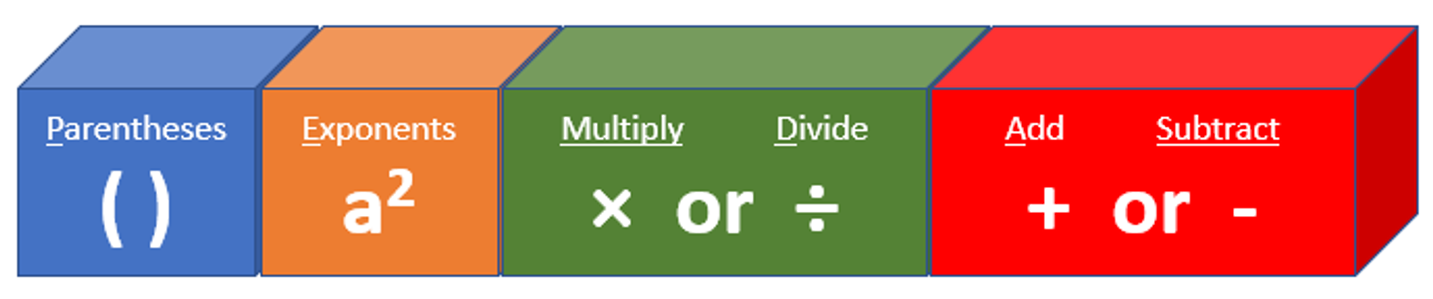
\includegraphics[width=\textwidth]{pemdas}
\centering
\end{figure}

ภาษา Python  ใช้สัญลักษณ์คำนวณทางคณิตศาสตร์ดังนี้  \cite{Bil15}

\begin{table}
\caption{สัญลักษณ์การคำนวณทางคณิตศาสตร์}
\centering
\begin{tabu}{l l l}
 \hline
 สัญลักษณ์คำนวณ & ชื่อการคำนวณ & ตัวอย่าง  \\ [0.5ex] 
 \hline
+ & บวก & a + b \\
- & ลบ & a - b \\
* & คูณ & a * b \\
/ & หาร & a / b \\
// & หารปัดเศษทิ้ง & a //  b \\
\% & เศษของการหาร & a \% b \\
** & ยกกำลัง & a ** b\\
\end{tabu}
\end{table}

\begin{codelist}{ตัวอย่างคำนวณทางคณิตศาสตร์}{}
>>> a
1
>>> b
2
>>> a + b
3
>>> a - b
-1
>>> b - a
1
>>> c = a - b
>>> c
-1
>>> a * b
2
>>> a * c
-1
>>> b * b
4
>>> b / a
2.0
\end{codelist}


\subsection{รูปแบบการเขียนการคำนวณทางคณิตศาสตร์แบบย่อ}

ในภาษา Python ผู้เขียนโปรแกรมสามารถเขียนการคำนวณทางคณิตศาสตร์แบบลดรูปหรือแบบย่อได้ 

\begin{table}[h!]
\caption{สัญลักษณ์การคำนวณทางคณิตศาสตร์แบบย่อ}
\centering
\begin{tabu}{l l l}
 \hline
 การคำนวณ & ตัวอย่าง & เทียบเท่ากับ  \\ [0.5ex] 
 \hline
+= & c += a & c = c + a \\
-=  & c -= a & c = c - a \\
*=  & c *= a & c = c * a \\
/=  & c /= a & c = c / a\\
//=  & c //= a & c = c // a \\
\%=  & c \%= a & c = c \% a \\
**=  & c **= a & c = c ** a\\
\end{tabu}
\end{table}


\subsection{การจัดการข้อความด้วยเครื่องหมายทางคณิตศาสตร์}

เครื่องหมายที่เป็นการคำนวณทางคณิตศาสตร์เมื่อถูกนำมาใช้กับข้อความ (String) จะเป็นอีกความหมายหนึ่ง เช่น การใช้เครื่องหมายบวกเชื่อมต่อระหว่างสตริง 2 ตัว หรือ การใช้เครื่องหมายดอกจันเป็นการเพิ่มสตริงเดียวกันตามจำนวนครั้งของการคูณ

\begin{codelist}{การจัดการข้อความด้วยเครื่องหมายทางคณิตศาสตร์}{}
>>> firstname
'Jantawan'
>>> lastname
'Piyawat'
>>> firstname + lastname
'JantawanPiyawat'
>>> firstname + '  ' + lastname
'Jantawan Piyawat'
>>> firstname * 3
'JantawanJantawanJantawan'
\end{codelist}


\section{Expressions และ Statements}

Expressions หมายถึงการใช้เครื่องหมายคำนวณและการใช้ตัวแปรและค่าของตัวแปรเพื่อหาผลลัพธ์ออกมา เอา Expression มาประกอบกันจะเรียกว่า Statement ดังนั้น Statement ก็คือคำสั่งเรียงต่อกันนั่นเองเพื่อใช้ในการสั่งงานคอมพิวเตอร์ด้วยภาษาคอมพิวเตอร์

\begin{codelist}{Expressions}{}
>>> 1+2
|3|
\end{codelist}

\begin{codelist}{Statements}{}
>>> c = a + b
>>> c
|3|
>>> print('hello world.')
|hello world.|

\end{codelist}


\section{การเขียนข้อความอธิบายโปรแกรมโดยการใช้ Comment}

Comment คือสิ่งที่เราเขียนใน Source Code ของโปรแกรมแต่คอมพิวเตอร์ไม่ต้องแปลผล เพื่อใช้ในการเขียนข้อความประกอบคำอธิบายในการสื่อสารระหว่างโปรแกรมเมอร์ด้วยกัน หรือเป็นการเตือนความจำของโปรแกรมเมอร์เอง โดย Comment ในภาษา Python นำหน้าด้วยเครื่องหมายชาร์ป (\#) แล้วหลังจากนั้นตามด้วยข้อความอะไรก็ได้ ถ้าจะเขียน Comment หลายๆ บรรทัดจะต้องใช้เครื่องหมายฟันหนู ('') หรือฝนทอง (')  3 ตัว แล้วก็พิมพ์ข้อความแล้วจึงปิดด้วยฟันหนู ('') หรือฝนทองทั้ง 3 ตัวอีกครั้ง (') ผลที่ได้จะมีเครื่องหมาย Backslash n (\textbackslash n) หมายถึงการขึ้นบรรทัดใหม่

\begin{codelist}{การใช้ Comment ในบรรทัดเดียว}{}
>>> print('Hello world!')
|Hello world!|
>>> # Hello how are you doing?
\end{codelist}

\begin{codelist}{การใช้ Comment ในหลายบรรทัด}{}
>>> x = '''
hello
1
2
3
'''
>>> x
'\nhello\n1\n2\n3\n'
>>> print(x)
hello
1
2
3
\end{codelist}


\section{Source Code}

ที่ผ่านมาเป็นการเขียนโปรแกรมแบบ Interactive คือเขียนบน Python Shell แล้วโปรแกรมจะแสดงผลออกมาได้เลย ซึ่งเรียกว่าการทำงานแบบ Interpreter เป็นการใส่คำสั่งไปที่ Prompt และ Python จะแสดงผลของคำสั่งนั้นออกมาเลย แต่ในความเป็นจริงแล้วจะเขียนโปรแกรมหลายๆ บรรทัดแล้วสั่งโปรแกรมทำงานทีเดียวพร้อมกัน เราจะเขียนไว้ในไฟล์นั้นเรียกว่า Source Code โดยที่ Source Code ของภาษา Python นามสกุลจะเป็น .py เวลาใช้ที่โปรแกรม Idle ให้กดที่เมนู File เลือก New เขียน Source Code แล้วให้กด Run ถ้าหากจะกดรันโปรแกรมอีกสักครั้งให้กด F5

\begin{codelist}{ตัวอย่าง Python Source Code}{}
x = 7
y = 6
if x == y: print('x and y are equal.')
else:
    if x < y: print('x is less than y.')
    else: print('x is greater than y.')
\end{codelist}

\begin{codelist}{ตัวอย่างผลลัพธ์ที่ได้จากการประมวลผล Source Code}{}
|x is greater than y.|
\end{codelist}


\section{คำสั่ง \texttt{print} (ตัวแปรหรือข้อมูล)}

print() เป็นฟังก์ชันที่ใช้ในการแสดงผลตัวแปรหรือข้อมูลออกทางหน้าจอ 

\begin{codelist}{คำสั่ง print()}{}
>>> print('Hello world!')
|Hello world!|
>>>
\end{codelist}


\section{การใช้คำสั่ง \texttt{input()} รับค่าจากแป้นพิมพ์}

คำสั่ง input(ข้อความ prompt) เป็นคำสั่งสำหรับรับข้อมูลจากผู้ใช้ด้วยการพิมพ์ผ่านแป้นพิมพ์ 

\begin{codelist}{คำสั่ง input()}{}
>>> name=input('What is your name? ')
|What is your name? Jantawan|
>>> print('Hello, ', name, end='.')
Hello, Jantawan.
\end{codelist}


\section{แบบฝึกหัด}

\begin{enumerate} 
\item จงหาเลขประจำตำแหน่งของข้อมูลต่อไปนี้
\begin{itemize}
\item love = 2
\item mom = “Jan”
\item wed = True
\item fah = 39.2 
\end{itemize}

\item จงหาประเภทของข้อมูลต่อไปนี้
\begin{itemize}
\item \pyinline{love = 2}
\item \pyinline{mom = 'Jan'}
\item \pyinline{wed = True}
\item \pyinline{fah = 39.2}
\item \pyinline{money = '22'}
\end{itemize}

\item จงแสดงผลต่อไปนี้
\begin{itemize}
\item ตั้งค่าตัวแปร dog, cat
\item แสดงข้อความ I have 3 dogs and 2 cats.
\end{itemize}

\item จงรับค่าจากผู้ใช้และแสดงผลต่อไปนี้
\begin{itemize}
\item ตั้งตัวแปร name 
\item รับค่าด้วยข้อความว่า กรุณาใส่ชื่อของคุณ
\item แสดงข้อความ สวัสดีค่ะคุณ
\end{itemize}



\item จงคำนวณหาค่าตัวเลขต่อไปนี้
\begin{itemize}
\item หาค่าพื้นที่สี่เหลี่ยม กว้าง 5 เมตร ยาว 3 เมตร
\item หาค่าพื้นที่สามเหลี่ยม สูง 5 เมตร ฐาน 3 เมตร
\end{itemize}


\item ให้ \pyinline{a = 3, b = 4, c = 5} จงหาค่าต่อไปนี้
\begin{itemize}
\item \pyinline{a == a*1}
\item \pyinline{a != b}
\item \pyinline{a > b}
\item \pyinline{b < c}
\item \pyinline{a+1 >= c}
\item \pyinline{c <= a+b}

\end{itemize}
\end{enumerate}








